\documentclass{article}

\usepackage[latin1]{inputenc}
\usepackage{tikz}
\usepackage{tikz-qtree}
\usetikzlibrary{shapes,arrows}

\usepackage{xspace}
\usepackage{graphicx}

\begin{document}
\pagestyle{empty}


\begin{figure*}
\begin{center}

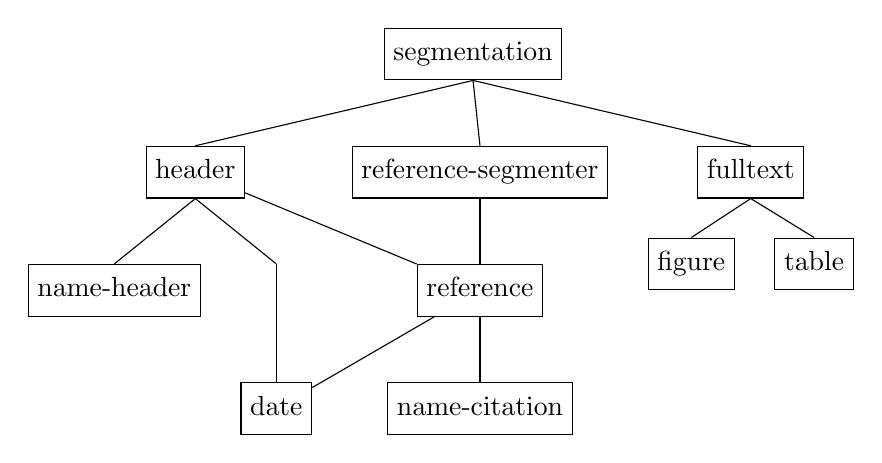
\begin{tikzpicture}[
  every tree node/.style={
    draw, 
%    inner sep=5pt, % space inside the nodes
    align=center,
    anchor=north,
    font=\strut},
  level 1+/.style={
    level distance=1.5cm,
    sibling distance=5mm},
  level 4+/.style={level distance=1cm} 
  ]
    \Tree [.\node(e0){segmentation};
            [.\node(e1){header};
                [.{name-header}
                ]
                [[.\node(e3){date};
                ]]
            ]
            [.{reference-segmenter}
                [.\node(e2){reference};
                    [.{name-citation}
                    ]
                ]
            ]
            [.{fulltext}
%                [.\node[below=auto,right=0.50cm](e5){figure};
                [.\node[right=0.50cm](e5){figure};
                ]
                %\edge[dashed,red] node[] {};
                  %[\edge[dashed,red] node[] {};
                    %[\edge[dashed,red] node[] {};
                      %[.\node(e4)[red]{recognition of software mention candidates};
                %]]]
                [.\node[left=0.50cm](e6){table};
                ]
            ]
        ]
    \draw (e1)--(e2);
    \draw (e2)--(e3);
    %\draw[dashed,red] (e5)--(e4);
    %\draw[dashed,red] (e6)--(e4);
    %\draw[dashed,red,semithick] (e5)..controls +(south est:1) and +(north west:2)..(e4);
    %\draw[dashed,red,semithick] (e1)..controls +(south est:1.5) and +(north west:1.5)..(e4);
    %\draw[dashed,red,semithick] (e0)..controls +(south est:4) and +(north west:0.1)..(e4);
    \end{tikzpicture}

  \caption{The GROBID cascade of sequence labeling models.}
  \label{grobid-cascade}
  
\end{center}
\end{figure*}

\end{document}
